\section{Vision Transformer (ViT) - An image is worth 16x16 words: Transformers for image recognition at scale} \label{appendix:vit-paper}

\subsection{Overview}

\par Dosovitskiy \textit{et al}, in their 2020 paper titled \textit{An image is worth 16x16 words: Transformers for image recognition at scale} \cite{vit}, aim to replace CNN based architectures with transformers for a multitude of computer vision tasks. They propose a transformer-based architecture inspired by Vaswani \textit{et al} \cite{tfm}, replacing the work embeddings with non-overlapping 'patch embeddings', extracted from images. The authors show that if ViT is pre-trained on large amounts of data, it can produce better results as compared to its CNN counterparts in various image recognition benchmarks.\par


\subsection{Datasets}
\begin{itemize}
\item Pre-trained on:
	\begin{itemize}
		\item ILSVRC-2012 ImageNet dataset with 1k classes and 1.3M images
		\item ImageNet 21k dataset with 21k classes and 14M images 
		\item JFT with 18k classes and 303M high-resolution images
	\end{itemize}
\item Benchmark tasks
	\begin{itemize}
		\item ImageNet (validation labels)
		\item CIFAR 10/100
		\item Oxford-IIIT Pets
		\item Oxford Flowers-102
		\item 19-task Visual Task Adaptation Benchmark (VTAB) classification suite.
	\end{itemize}
\end{itemize}


\subsection{Performance}
\par Dosovitskiy \textit{et al} report state-of-the-art-performance for various image recognition tasks (datasets mentioned above), when compared with current state-of-the-art models such as Big Transfer (BiT) \cite{bit} and Noisy Student \cite{nos}.\par


\subsection{Methodology}

\par Dosovitskiy \textit{et al} use the original transformer model \cite{tfm}, but with different input embeddings that are extracted from images. The transformer model then outputs a classification ([class]) token which represents the entire image. This [class] token is then used for downstream tasks (mentioned above).\par

\begin{figure}[h]
	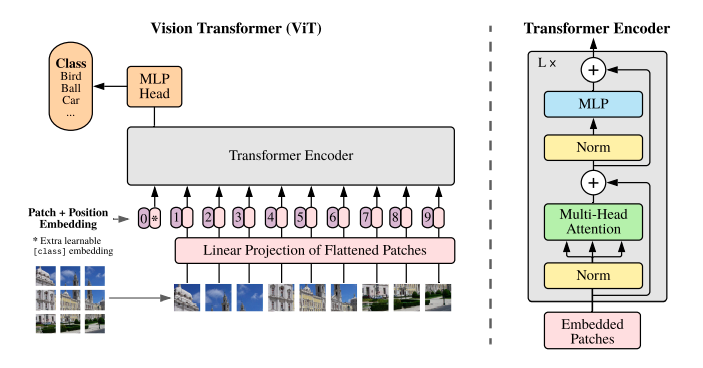
\includegraphics[width=\linewidth]{assets/img/vit.png}
	\caption{Video Transformer introduced by Dosovitskiy \textit{et al} (Image courtesy \cite{vit})}
\end{figure}


\subsubsection{Input: Patch embeddings}

\par The input consists of flattened $nxn$ patches of an image. These patches are non-overlapping and span the entire image. 
\begin{itemize}
	\item The original image $x = R^{H \times W \times C}$.
	\item This is converted to a flattened 2D patch $x_p = R^{N \times (P^2 \cdot C)}$ where $H \times W$ is the resolution of the image, $C$ is the number of channels, $P \times P$ is the resolution of each patch.
	\item $N = HW / P^2$ represents the number of patches extracted from the image and serve as the sequence length for the transformer. These are the patch embeddings.
	\item Position embeddings are added to the above patch embeddings. These can be:
	\begin{itemize}
		\item 1D, like in transformers.
		\item 2D, based on row and column indices.
		\item Relative distances between patches to capture the true spatial positioning of each patch within the image.
	\end{itemize}
	\item A learnable [class] token is prepended to the image sequence like the BERT model. $z_0$ is the input [class] token and $z_l$ is the output token. $z_l$ is a vector that represents the entire image and can be used for downstream tasks.
	\item These embeddings are mapped onto a D-dimensional space which is used by the encoder (ViT).
\end{itemize}
\par

\subsubsection{Transformer Encoder}

\par The transformer model proposed in \cite{tfm} is inherently the same one used by ViT. The only difference is that a normalisation layer is added before the multi-headed self attention block. Additionally, ViT used the GELU non-linearity as part of the multi-layer perceptron block. \par

\begin{figure}
	\centering
	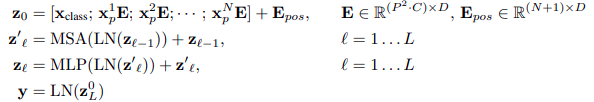
\includegraphics[width=\linewidth]{assets/img/vit-eq.png}
	\caption{Video Transformer introduced by Dosovitskiy \textit{et al} (Courtesy \cite{vit})}
\end{figure}


\subsubsection{Training Procedure}
\par Pretrained on datasets such as ImageNet, ImageNet-21k, JFT-300M for better performance.
\begin{itemize}
	\item Adam optimizer with $\beta_1$ = 0.9, $\beta_2$ = 0.999, batch size = 4096, weight decay = 0.1
	\item Strong regularization is used throughout the encoder. Dropout, when used, is applied after every dense layer except for the the query-key-value projection layers and directly after the addition of positional embeddings
	\item Training is done on a resolution of $224 (14 \times 14)$
\end{itemize}

\subsection{Conclusion}
\par The work by Dosovitskiy \textit{et al} provides a compelling case for using transformers instead of CNN-architectures in image recognition tasks. Even though it requires large amount of pre-training, it can be scaled much better than its CNN counterparts and can meet the performance (and even exceed it in certain cases) of current state-of-the-art CNN-based models.
